\section{Introduction}
\label{sec.introduction}


% Start of the outline
%\par
%\textbf{Outline:}
%\begin{itemize} 

%\item Kernel vulnerability is a serious problem that has not been solved, in spite of large amount of efforts devoted by researchers and practitioners.  

%\begin{itemize} 
%\item The number of kernel vulnerabilities is growing substantially, as the size of the kernel is increasing continuously.  

%\item The serious damage and harm caused by kernel vulnerabilities
%\begin{itemize} 
%\item The economic and political damage incurred by kernel vulnerabilities. (the huge impact of this problem)
%\item Technical problems caused by kernel vulnerabilities. (specific problems caused by kernel vulnerabilities)
%\end{itemize}

%\item Many Linux kernel vulnerabilities are hidden. For example, many Linux kernel vulnerability patches were undocumented, leaving users have to guess many of the vulnerabilities fixed or not. [http://arstechnica.com/security/2013/05/critical-linux-vulnerability-imperils-users-even-after-silent-fix/]

%\item It is very easy to trigger the kernel vulnerabilities. Since the kernel provide an interface, which is rich and exploitable. Untrusted code and applications could touch the kernel and trigger vulnerabilities. 
%\end{itemize}

%\item Bugs in benign applications or malicious code will target and trigger kernel vulnerabilities. 

%\item We want to run applications, while minimize the potential danger of triggering kernel vulnerabilities. 
%\end{itemize}
% End of the outline


\par
The operating system (OS) kernel has always been an appealing target.
During the past few years, the exploitation of OS kernels has become a very
serious problem that remains to be solved, in spite of large amount of
efforts devoted by researchers and practitioners. There were 125 reported
vulnerabilities of the Linux kernel \cite{CVE:14} (Figure 1), and 215
reported vulnerabilities of all kinds of kernels in 2014 \cite{NVD:14}.
Admittedly, the exploitation of user-level software has become much harder,
as recent versions of popular OSes come with numerous protections and
exploit mitigations. The principle of least privilege is better enforced in
user accounts and system services, compilers offer more protections against
common software flaws, and highly targeted applications, such as browsers
and document viewers, have started to employ sandboxing technique. On the
other hand, the kernel has a huge codebase and an attack surface that keeps
increasing due to the constant addition of new features \cite{Metrics:13}.
Indicatively, the size of the Linux kernel in terms of lines of code has
more than doubled, from 6.6 MLOC in v2.6.11 to 16.9 MLOC in v3.10
\cite{Linux:13}.


\begin{figure}[h]
\centering
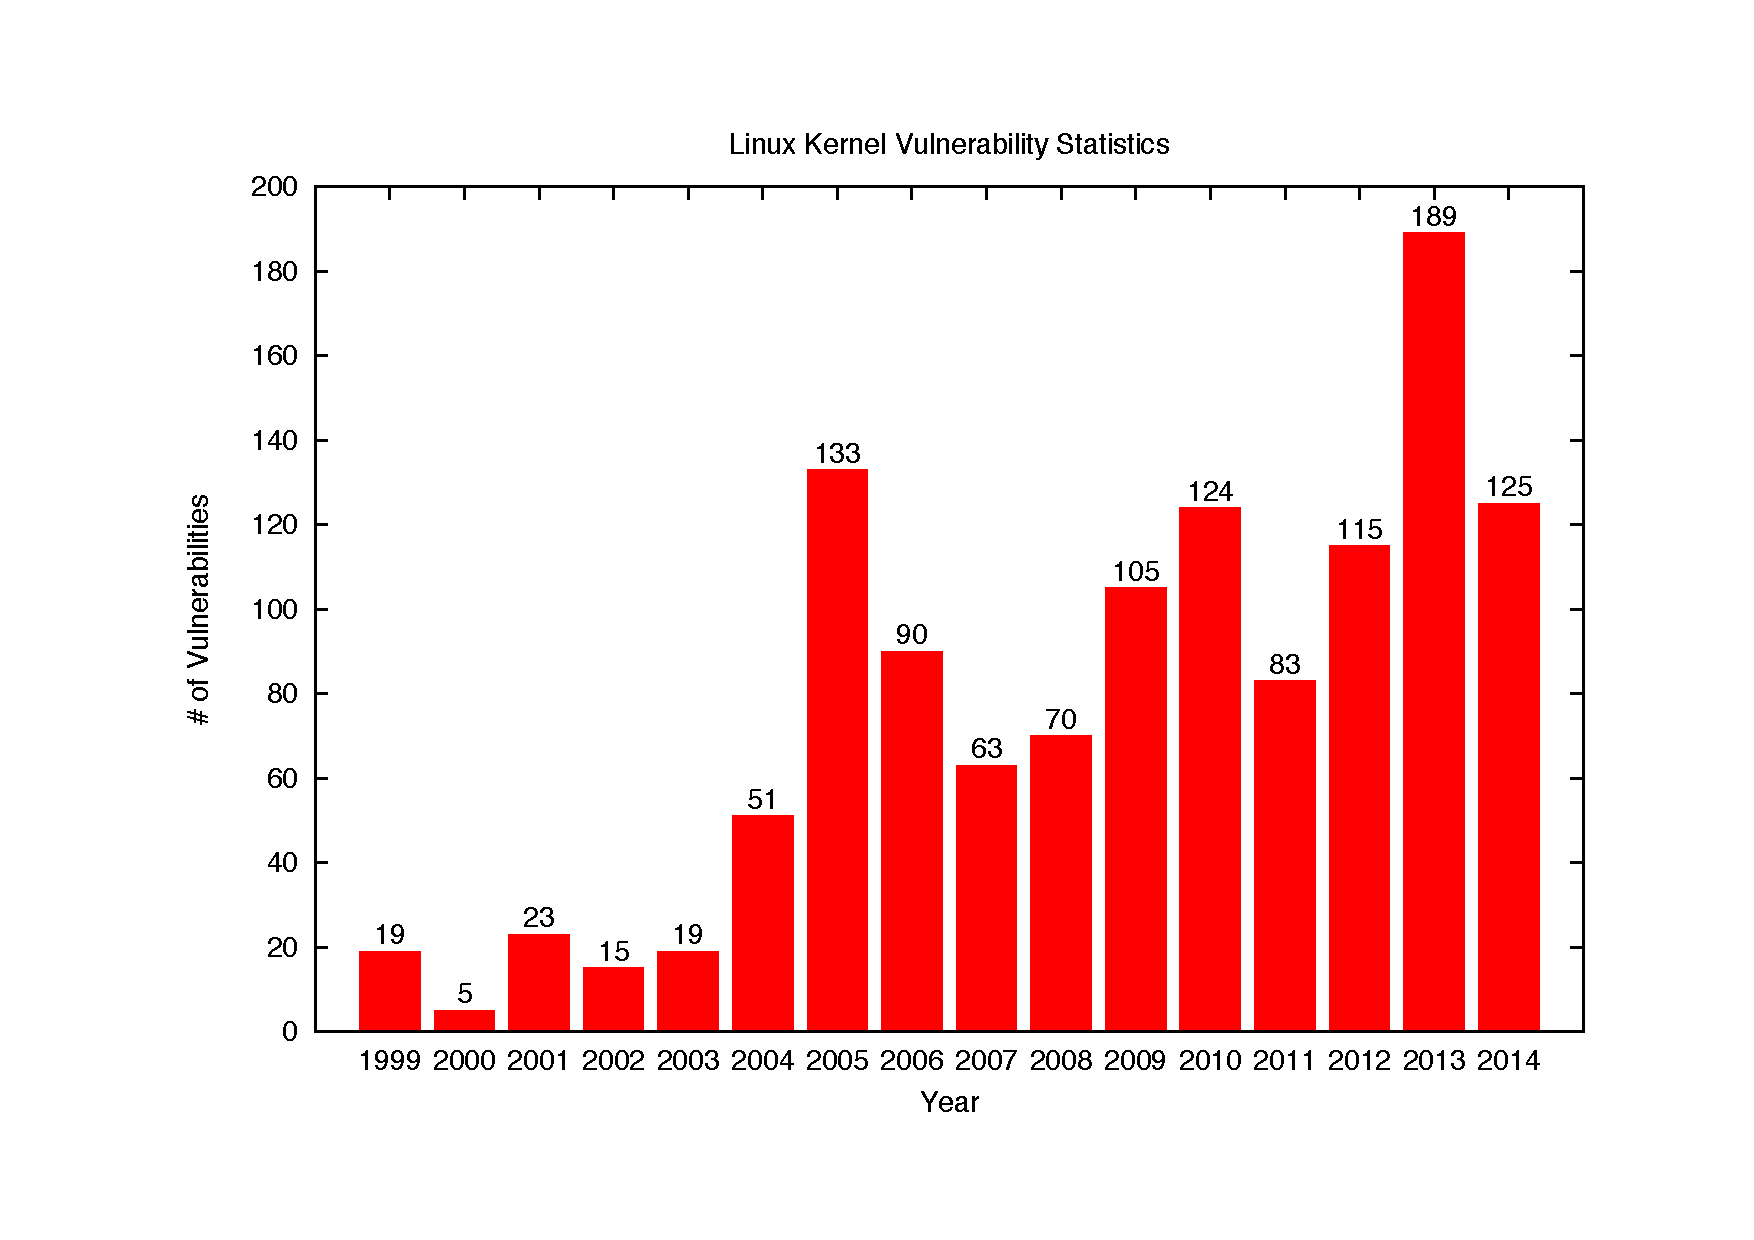
\includegraphics[width=1.0\columnwidth]{diagram/linux_kernel_vul_total_stats.pdf}
\caption{Linux Kernel Vulnerability Statistics }
\label{fig:arch}
\end{figure}


\par
Opportunities for kernel exploitation are abundant. As an example consider
the Linux kernel, which has been plagued by common software flaws, such as
stack and heap buffer overflows \cite{CVE:20093234, CVE:20131828,
CVE:20132892}, NULL pointer and pointer arithmetic errors
\cite{CVE:20050736, CVE:20092698}, memory disclosure vulnerabilities
\cite{CVE:20093002, CVE:20104073}, use-after-free and format string bugs
\cite{CVE:20132852, CVE:20134343}, signedness errors \cite{CVE:20103437,
CVE:20132094}, integer overflows \cite{CVE:20050736, CVE:20102959}, race
conditions \cite{CVE:20091527, CVE:20093547}, as well as missing
authorization checks and poor argument sanitization vulnerabilities
\cite{CVE:20103904, CVE:20104347, CVE:20120946, CVE:20130268}. The
exploitation of these bugs is particularly effective, despite the existence
of kernel protection mechanisms, due to the weak separation between user
and kernel space.


\par
The key problem is that kernels provide a system call interface, which is
rich and exploitable. Proper protection of the interface between untrusted
user applications and the kernel becomes essential. Previous efforts
attempt to address the problem by either filtering and blocking the unsafe
system calls (``check-and-pass-through''), or by moving some of the system
functionality outside the kernel to provide a library OS
\cite{Drawbridge:11} (``re-implement''). However, both approaches still
allow untrusted applications to have access to substantial kernel
footprint. As a result, there are still plenty of chances to trigger bugs
hidden in the underlying kernel.


%\par
%A common lesson from computer security is that bugs are prevalent in code,
%especially large and complex pieces of code like an operating system
%kernel. Buggy code could cause serious problems. Bugs in applications
%could trigger faults in operating system kernel. Faults in the OS kernel
%or other trusted operating system code, pose a serious risk to all
%software on the device. To reduce damages caused by bugs, many helpful
%techniques for bug finding are created and used. However, researchers and
%hackers are still increasingly finding bugs in essentially all widely
%deployed programs. We are facing a serious problem: with the existence of
%bugs, is it possible to execute applications yet minimize potential
%damage?


%\par
%This problem has not gone unnoticed by the computer security community.
%Substantial effort has been devoted to executing applications safely.
%Virtualization is widely used to isolate untrusted applications that share
%the same hardware. There is bare metal hardware virtualization, such as
%VMware ESX Server, XEN, and MS Hyper-V. There is also hosted hardware
%virtualization, such as VMware Workstation, VMware Server, MS Virtual PC
%and Server. However, there are limitations with virtualization.
%Virtualization hypervisor suffers from attack vectors including
%architectural vulnerability, software vulnerability, and configuration
%risk. For example, small code footprint of hypervisor could become a
%potential vulnerability and lead to serious problem.


\par
Recently, many researchers develop systems that adopt a
``check-and-pass-through'' security model. These systems employ trusted
code which monitors and restricts the set of system calls a program is able
to execute. If an application issues an untrusted call, it is blocked and
thus prevented from causing harm. The rationale is that if access to
``unsafe'' calls is denied, applications can execute the other system calls
securely on the underlying operating system. Such
``check-and-pass-through'' model is typically implemented via system call
interposition, a method that regulates and monitors application behavior.
This approach can be thought of as a firewall that is between the
application and the OS, regulating which calls are safe and allowed to
pass. The system call interface is a boundary that can permit or deny
application interaction with file system, network, and other sensitive
resources. Such an interface is crucial, but complex to understand. Simply
monitoring it can potentially lead to a range of pitfalls if any minor
details are overlooked. For example, a symbolic link race could occur when
the link is modified between the time the symbolic link is checked, and
when an access relying on that check occurs. If this link is modified to
pointed to a file that has restricted accessing properties in the system,
then accessing this sensitive file through the symbolic link will be
allowed by the ``check-and-pass-through'' approach. Meanwhile,
``check-and-pass-through'' must obtain and interpret OS state associated
with the application to make policy decisions. This is usually achieved by
OS state replication. However, replicating the OS state can easily lead to
state inconsistency and thus result in incorrect decision. Changes needed
to take care of these details are usually significant and expensive.


\par
Another alternative, which we call the ``re-implement'' method, is to
recreate the functionality of the OS as a user process (e.g. VirtualBox,
VMWare workstation). However, in practice the resulting systems are not
secure because the virtual machine monitor for such a system still has
access to the underlying OS kernel through the system call interface --- a
rich and exploitable interface.


\par
In this paper, we propose a new model for isolating untrusted code called
the ``safely-reimplement'' method. As before a sandboxed client program
executes and passes its calls to a monitor.  However, in this model,
wherever possible the requested functionality is re-implemented in a safe
way within the monitor. This implementation is done inside of a safe
dual-layer sandboxed programming environment, which itself is optimized to
have a small trusted computing base. This approach minimizes the portions
of the kernel accessible to untrusted code. For example, many programs
create, remove, and move directories as part of their normal operation.
There are many ``time-of-check-to-time-of-use'' (TOCTTOU) vulnerabilities
that have historically appeared in kernels and security systems with the
way that directory traversal is handled. With ``check-and-pass-through'',
the monitor asks the kernel to create directories. Thus an attacker that
can create directories can trigger a flaw in the kernel and exploit the
flaw. In a ``safely-reimplement'' system, the monitor implementation
handles the concept of directories by writing metadata into one or more
regular files on the file system. The only kernel paths that are touched
include common calls like file open, read, write, and close. Furthermore,
the set of arguments used for each call is also highly restricted. Thus,
all open calls will involve a file name in the local directory, with the
one, constant set of flags needed by the monitor. As a result, the kernel
is touched infrequently and is only touched in commonly used paths where it
is more likely that TOCTTOU bugs would have been uncovered.


\par
If a bug does exist in the monitor this also has different impacts for each
design. With ``check-and-pass-through'' model, the monitor code is trusted.
Thus a bug in this code often results in access to a sensitive part of the
kernel, potentially allowing escape of the sandbox. In fact, since the
monitor code is often located in the kernel, a flaw that breaks memory
safety usually allows arbitrary compromise of the system. In the
``safely-reimplement'' model, the monitor implementation is a program
executing in a contained environment. If a flaw exists, it is exhibited as
a problem with the environment the application runs in rather than an
exploitable kernel flaw. For example, consider a bug with symbolic link
handling in a monitor. The operating system may treat such files as unique
and the monitor may be confused and feel they are distinct. If a
``check-and-pass-through'' monitor handles this situation poorly, it may
result in bypassing security restrictions the monitor is meant to enforce.
However, a ``safely-reimplement'' monitor with the same flaw will not rely
on the kernel code paths for symbolic links. The monitor will implement the
(incorrect) behavior, but do so within code running in a sandbox. Since the
monitor does not have privileged access to the system as the kernel does,
this will not result in a security issue. The usual outcome of a bug in
this case is to cause the application to fail (due to reliance on behavior
that does not occur), instead of security escape.


\par
Similarly, the way that a monitor handles kernel functionality that is
unknown to the authors also differs. For example, the monitor authors may
be unaware of an additional option or flag for a system call. In the
``check-and-pass-through'' monitor, this monitor author may unintentionally
allow an attacker to reach this functionality, which may pose a security
risk. (This is analogous to the `fail-open' security principle.)  In a
``safely-reimplement'' monitor, since the monitor must implement
functionality for it to exist, the monitor will not support the unknown
functionality. So unknown functionality cannot possibly be exposed by the
monitor author. (Much like the `fail-closed' security principle.) As a
result, the application does not present a security risk.


\par
Based on our new ``safely-reimplement'' model, we designed and implemented
our system, Lind, which securely reconstructs complex yet essential
operating system calls inside a sandbox. Lind provides user applications
with a rich and sufficient POSIX API, while only allowing minimum contact
with the kernel. We ran legacy applications, such as Tor and Apache, in
Lind. Our evaluation shows that legacy applications running in Lind have
good performance. Furthermore, applications running in Lind were well
isolated from other parts of the system. Untrusted user applications only
touched a small portion of commonly used kernel code, and will not trigger
severe kernel bugs.


\par
In summary, the contributions of this paper are as follows:

\begin{itemize} 
  
  \item We proposed a new ``safely-reimplement'' model for isolating
untrusted code. Operating system functionality is reimplemented safely
within our dual-layer sandbox, which itself is optimized to have a small
trusted computing base.
  
  \item Based on our ``safely-reimplement'' model, we designed and
implemented Lind, a portable, lightweight, and single-process sandbox,
which provides a safe 
environment for executing programs and controlling resource usage at the
process granularity.
  
  \item We conducted performance evaluation of Lind. Legacy applications,
such as Tor and Apache, ran unmodified in Lind. Under benchmark included in
the Tor source code, Lind slowed the operations down between 2.5x and 5x.
Furthermore, we conducted security evaluation. Only a small portion of
kernel code was reached and triggered by common applications tested. Kernel
was touched infrequently and only in commonly used paths, which limited the
risk of triggering undetected bugs in the kernel.

\end{itemize}


\par
The rest of this paper is organized as follows. We discuss our threat model
and background information on two existing technologies we leveraged in
Section 2. Architecture of our work is introduced in Section 3. Evaluation
results are presented in Section 4. We then discuss related work in Section
5 and conclude in Section 6.
